\chapter{Metodologia}
\label{cap:metodologia}
 Este capítulo descreve a nossa proposta de visualização para exploração dos
fluxos no tráfego de veículos. O objetivo principal da visualização é centrado
nas propriedades espaciais e temporais dos dados para entender como são os
fluxos de origem e destino pela cidade ao longo do tempo. Buscamos um maior
nível de detalhes através de uma abordagem multinível para explorar padrões
globais e locais do tráfego, com diferentes níveis de agregação temporais e
espaciais.

 Apresentamos inicialmente a ferramenta que iremos utilizar para responder às
questões de pesquisa levantas no Capítulo \ref{cap:introducao}, e que
relembramos a seguir. Damos uma visão geral dos seus componentes e dos
artefatos de entrada e saída que irão resultar na visualização e possibilitar a
análise dos dados. A ferramenta faz parte do ecossistema de soluções para
cidades inteligentes que são desenvolvidas no contexto do projeto
InterSCity\footnote{\rurl{interscity.org}}. Em seguida detalhamos os conjuntos
de dados que iremos utilizar e suas características, e por fim, explicamos as
técnicas que pretendemos aplicar para destacar as propriedades dos dados dentro
de uma visualização para responder às nossas questões:

\begin{itemize}
  \item \textbf{Q1:} Como o \emph{bundling} pode ser usado para identificar os
fluxos de origem e destino no trânsito em diferentes escalas?

  \item \textbf{Q2:} É possível utilizar o \emph{bundling}  para
identificar padrões de fluxos de origem e destino no trânsito?

  \item \textbf{Q3:} O \emph{bundling} é eficiente para gerar uma
visualização de uma grande quantidade de dados do trânsito?
\end{itemize}

\section{Implementação da Visualização}
  Poucos algoritmos de \emph{bundling} são implementados em bibliotecas de uso
aberto. A maioria dos trabalhos pesquisados não disponibilizam a fonte para as
suas ferramentas e implementação dos seus algoritmos, e ainda que os algoritmos
estivessem disponíveis seria necessário implementar a ferramenta para
visualizar os dados da forma como queremos. Optamos então por partir de uma
implementação própria para a visualização dos dados, apoiando-nos em
bibliotecas já existentes para exploração de dados geoespaciais.

  Apresentamos o InterSCityPlotter, uma ferramenta para análise de dados do
tráfego que permite a criação de múltiplas visualizações, como visualizações
estáticas (Figura \ref{fig:simulated-traffic}) e visualizações baseadas em
pontos pontos (Figura \ref{fig:rastro}).  O objetivo da ferramenta é dar
suporte a estudos com dados do trânsito gerados pelo InterSCSimulator e também
por outras fontes, com o propósito de abranger análises de dados geoespaciais
que representam deslocamentos de um ponto de origem até um ponto de destino. O
diagrama da Figura \ref{fig:interscityplotter} mostra uma visão geral dos
componentes da ferramenta os quais damos uma breve descrição em seguida.

\begin{figure}[!htb]
  \centering
  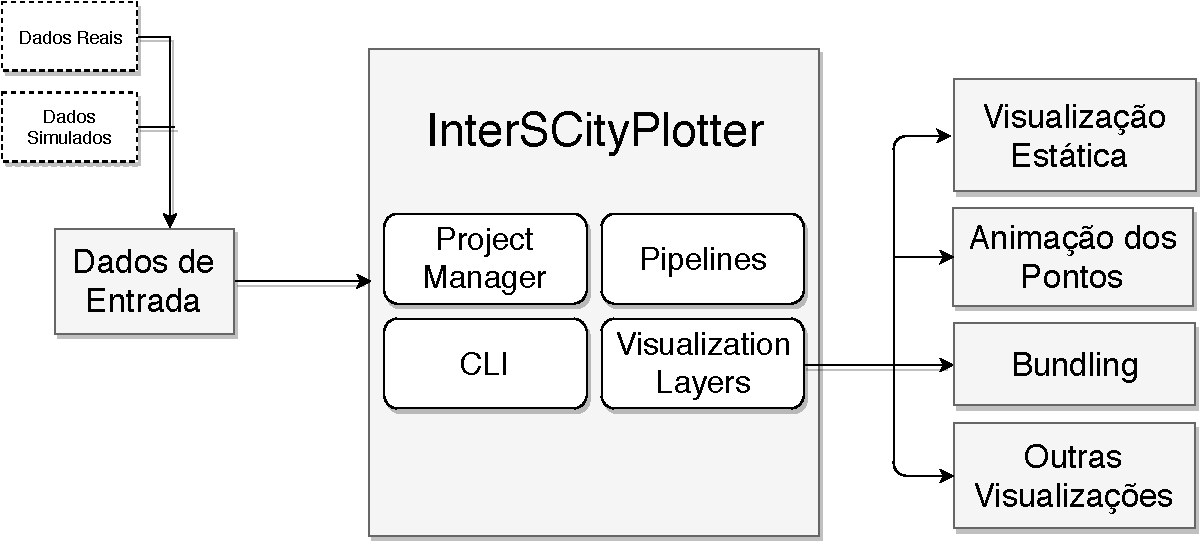
\includegraphics[width=1\textwidth]{../figuras/interscityplotter.pdf}
  \caption{Visão geral da arquitetura da ferramenta InterSCityPlotter.}
  \label{fig:interscityplotter}
\end{figure}

\begin{description}
\item[\emph{ProjectManager}:] a exploração de dados do tráfego começa com a
criação de um novo projeto de visualização a partir de um conjunto de dados de
entrada. Esse componente é responsável pela criação, exclusão e outras ações de
gerenciamento dos projetos. Para utilizar a ferramenta, é necessário criar um
novo projeto apontando o conjunto de dados em um formato CSV. Os dados irão
passar por algumas etapas de pré-processamento definidos no componente
\emph{Pipelines} para que estejam prontos para visualização junto com os
arquivos do projeto criado.

  \item[\emph{Pipelines}:] esse componente isola as etapas de pré-processamento
necessárias para uso dos dados nas visualizações, como por exemplo limpeza e
checagem de inconsistências, derivação de novos atributos, etc.  Outras ações
também são definidas nesse módulo, como por exemplo, uma análise inicial que
contabiliza o número de trajetórias, quantidade média de pontos por trajetória
e número total de pontos no conjunto de dados é feita assim que se cria um
projeto. Essas informações são salvas junto com os dados do projeto.

  \item[VisualizationLayers:] o componente \emph{VisualizationLayers} baseia-se
na biblioteca Geoplotlib, apresentada em \citet{Andrea2016}, que fornece
recursos para criação de visualizações de dados geoespaciais. Ela fornece todo
o arcabouço em baixo nível para renderização de imagens a partir desses dados e
possui também algumas visualizações pré-definidas para projetar pontos e linhas
em um mapa. Os recursos do Geoplotlib serão estendidos dentro do
InterSCityPlotter para a implementação de diferentes tipos de visualizações
(Layers) customizadas. A visualização com \emph{bundling} que propomos será
construída como uma nova \emph{layer}.

  \item[CLI:] o módulo CLI possui a lógica para interação com a ferramenta
através da linha de comando. Essa interação se resume atualmente a comandos de
gerenciamento dos projetos (criação, exclusão) e execução de uma das
visualizações já desenvolvidas. A documentação completa pode ser vista no
repositório da ferramenta, disponível no
Github\footnote{\rurl{github.com/tallysmartins/interscity-plotter}}.
\end{description}

  A ferramenta se encontra em processo de desenvolvimento. Os módulos
\emph{Project Manager}, \emph{Pipelines} e CLI já estão parcialmente
implementados e já é possível criar um novo projeto a partir de dados do
simulador, que posteriormente passam por um primeiro pré-processamento para
contabilizar algumas estatísticas, como número de veículos totais, média de
pontos por viagem, tempo total da simulação e outros. Ainda restam implementar
todo o módulo \emph{VisualizationLayers} e também alguns pré-processamentos do
módulo \emph{Pipelines} que iremos utilizar para tratamento dos dados de
entrada e derivação de novos atributos.

\section{Conjuntos de Dados}
   Os dados do tráfego que utilizaremos possuem o registro da posição e o tempo
ao longo de toda a trajetória, desde a origem até seu destino. Outros atributos
como velocidade, direção, aceleração, podem ser derivados a partir dos dados
brutos. Cada trajetória $T$ de um veículo pode ser modelada como uma sequência
de pontos $p_i$ que contém a sua posição, o instante de tempo e um vetor $a$
contendo outros $n$ possíveis atributos. Em nosso estudo, esse vetor guarda a
direção, dada pelo ângulo da reta entre os pontos de origem e destino de cada
trajetória.

\begin{center}
$T = \left\langle p_i = ((latitude, longitude) \in \mathbb{R}^2, t \in \mathbb{R}^+, a^n \in \mathbb{R})_i \right\rangle$
\end{center}

  Duas fontes de dados com informações do tráfego de veículos na cidade de São
Paulo serão usadas neste trabalho. A primeira é uma API pública disponibilizada
pela prefeitura da cidade e que fornece dados da movimentação dos ônibus. A
outra fonte é o simulador InterSCSimulator, o qual usaremos para obter dados
do tráfego.

\subsection{Tráfego dos Ônibus de São Paulo} São Paulo possui uma frota de
cerca de 15 mil ônibus que circulam diariamente nas vias da cidade e fazem mais
de 70 mil viagens por dia em mais de 2 mil linhas diferentes. A posição dos
ônibus durante seu percurso é registrada a cada 45 segundos com aparelhos de
GPS e disponibilizada pela Secretaria de Transporte Público
(SPTrans)\footnote{\rurl{www.sptrans.com.br/desenvolvedores/APIOlhoVivo/Documentacao.aspx?1}}
através de API pública. As buscas dos dados são feitas pelo código da linha,
que retorna naquele momento informações de todos os veículos daquela linha em
operação nas ruas, retornando o código do veículo, horário da coleta, posição
(latitude e longitude) e se o ônibus possui suporte para pessoas com
deficiência. A lista de todas as linhas existentes também podem ser adquiridas
pela API.  A Listagem \ref{olhovivo.json} mostra um exemplo de uma consulta na
API para a linha de ônibus 2023. Mais detalhes podem ser vistos na documentação
da API que fornece os dados.

\begin{lstlisting}[style=myxml, caption={Parte da resposta obitida para a linha 2023}, label=olhovivo.json]
{
 "hr"=>"14:25", // Hora da requisição
 "vs"=> [       // Lista de ônibus em circulaçao
   {
    "p"=>"82324", // Identificador do veículo
    "a"=>true,    // Acessível a deficientes
    "ta"=>"%*2019-01-30T16:25:05Z*)", // Hora da coleta dos dados em formato UTC
    "py"=>-23.562566125000004, // Latitude
    "px"=>-46.72267612500001   // Longitude
   }]
}
\end{lstlisting}

Para a visualização do tráfego serão coletados os dados de um dia do tráfego de
ônibus. Embora não representem a totalidade do tráfego, esses dados compõe uma
grande parte da movimentação que ocorre na cidade ao longo do dia e servem como
base para comparação com a visualização dos dados simuladas. Pretendemos
explorar em nossa análise os padrões de movimentação no trânsito, como regiões
de maior fluxo e como ele se comporta em diferentes momentos do dia, como
horários de pico.

\subsection{Tráfego Simulado de Veículos}
  O uso de dados simulados nos trazem dois aspectos importantes levantados em
nossas questões \textbf{Q2} e \textbf{Q3}. O primeiro é a possibilidade de
obtermos cenários diferentes do trânsito com alterações na simulação, já o
segundo aspecto é capacidade de obtermos uma grande quantidade de dados do
tráfego de veículos no trânsito.

  Utilizaremos uma simulação do tráfego de carros e ônibus na cidade de São
Paulo com cerca de 585 mil veículos. O cenário foi criado e disponibilizado por
\citet{santana2018courb} e gerou um arquivo de saída com mais de 31 milhões de
eventos de movimentação dos veículos. Para construir o arquivo de entrada
\emph{trips.xml} com as mais de 585 mil viagens, eles utilizaram uma matriz de
Origem-Destino (OD) feita pela Companhia do Metropolitano de São Paulo
(Metrô)\footnote{Pesquisa Origem-Destino - \rurl{goo.gl/DNM8in}} que pesquisou
como os cidadãos se locomovem pela cidade e usaram isso para determinar a
movimentação dos carros.  Além disso, utilizaram também dados dos itinerários
dos ônibus fornecidos pela SPTrans para estabelecer viagens de ônibus com
horários, paradas e frequência mais realistas.

  A pesquisa OD catalogou 160 mil amostras de viagens realizadas em um dia de
semana da cidade de São Paulo. Ela possui dados como a origem, o destino, a
hora de início, o modo de transporte e um fator a extrapolação estatística dos
dados usado para generalizar os valores da amostragem para toda a cidade.
Destas viagens, cerca de 26 mil são feitas de carro, como mostram
\citet{santana2018courb}. Utilizando o fator máximo de extrapolação da pesquisa
é possível chegar a uma quantia de mais de 4 milhões de viagens de carro e
ônibus em um dia, mas é possível realizar simulações menores reduzindo esse
fator. Posteriormente, fazemos alterações no arquivo \emph{map.xml} para
alterar o comportamento da simulação e obter um cenário diferente, que
comparamos com o cenário original. Detalhamos essas alterações na Seção
\ref{sec:vis-eventos}.

\subsection{Pré-processamento dos dados}

  Os dados coletados estão sujeitos a erros, e por isso, algumas etapas de
pré-processamento são necessárias. O módulo de \emph{Pipelines} da ferramenta
InterSCityPlotter é o local destinado a armazenar as rotinas que fazem essas
manipulações dos dados, tanto de limpeza quanto de derivação de novos
atributos. Mapeamos as seguintes rotinas para tratamento dos dados:

\begin{description}
  \item[Viagens da simulação não finalizadas:] isso pode ocorrer
quando o tempo da simulação acabado e uma viagens ainda está no meio do percurso,
essas viagens devem ser identificadas e removidas da análise.

  \item[Dados inconsistentes com a trajetória:] os dados dos ônibus fornecidos
pela prefeitura podem conter inconsistências devido a erros nos sensores e/ou na transmissão,
como por exemplo, pontos fora das vias. Esses dados devem ser identificados e removidos da análise.

  \item[Rotas circulares:] alguns ônibus têm rotas circulares, ou seja, o ponto
de partida e de chegada são o mesmo. Deve-se observar esses casos e seus efeitos
na visualização, para se necessário, removê-los.

  \item[Anomalias:] podem ocorrer que algumas trajetórias apresentem uma distância
muito pequena, ou pontos esparsos. Essas possíveis anomalias devem ser identificadas
e removidas da análise.

  \item[Derivação da direção:] esse atributo será derivado a partir dos pontos
de origem e destino de cada trajetória e será dado por um ângulo $\theta$ no
plano cartesiano dado pelas latitudes e longitudes do globo.
\end{description}

  Outras necessidades de pré-processamento podem surgir ao longo da pesquisa.
Estes são apenas itens já identificados até o momento, e que receberão atenção
durante o processo de implementação da visualização.

\section{Visualização}

  Explorar todas as possibilidades seria um trabalho extensivo. Focamos
então em algumas classes de problemas dentro da visualização de dados
com bundling para explorar o seu potencial na análise de fluxos de origem e
destino na cidade.

\subsection{Explorando propriedades espaciais - coisas óbvias}

- Aplicar o bundling para ver regiões densas, conforme mostrados na OD
	x) Mostrar as features de cores padrão (distância, direção, densidade)
	x) Mostrar as features de cores implementadas (tipo de transporte, modo de transporte, renda, gênero)
	x) Mostrar que tem pessoas que andam de metrô em locais que não tem metrõ (adicionar mapa)
	x) Mostrar como os ônibus metropolitanos se interceptam com os de são paulo
	x) Mostrar que os filtros de dados por horário pra mostrar que há mais fluxo
		 no horário de pico, que os onibus escolares saem todos pela manhã, mas que também temos
		pessoas que saem de madrugada para trabalhar
	x) Mostrar a renda e correlacionar distância do centro com renda
	x) Mostrar correlação de renda com carro (pobre anda de carro?)
	x) Derivar um atributo do quão o horário de pico afeta e usar como VALUE

	- Quais vantagens e desvantagens em relação ao que existe na OD (substitui alguma coisa do relatório da OD?)
	- Qual o nível de detalhes conseguimos extrair alguma informação?

  
\subsection{Estratégias de bundling}

2) Mostrar a mesma grandeza de diferentes maneiras
- Grandezas: Tempo/Tipo de transporte/Direção
- Estratégias: Fazer bundle de tudo e aplicando filtro E cores vs separado, diferenciar por cores no bundling de tudo, e filtrar as arestas no tempo (manhã e tarde)
	x) Fazer bundling de todos os dados de transporte e filtrar por modo
	x) Fazer bundling de todos os dados de transporte e colorir por modo
	x) Fazer bundling dos modos de transporte separados
	x) Fazer bundling dos dados em direção opostas

	Vantagens e desvantagens em relação aos gráficos da OD?
	Qual os níveis de detalhes conseguimos obter?

\subsection{Agregação Espacial Multinível}

3) Escalar o agrupamento conforme o zoom e resolução diferentes e dados diferentes (tunning não muito óbvio)
	- Número de pontos
	- Resolução da imagem
	- tamanho do kernel
	- Glanuralidade dos dados
	x) Aplicar bundling com alta resolução e alto numero de pontos, kernel grande e kernel pequeno
	x) Aplicar bundling com alta resolução e baixo numero de pontos, kernel grande e kernel pequeno
	x) Aplicar bundling com baixa resolução e alto numero de pontos, kernel grande e kernel pequeno
	x) Agrupar os dados na mão em regiões e aplicar o bundling em macro regiões. Qual a alguma diferença?
	x) Mostrar o bundling dos dados dos centróides e dos dados específicos em alguns modais (metrô, a pé, bike, taxi)

	Explicar que não há uma métrica, mas dissertar sobre qual fica melhor visualmente
	- Vantagens e desvantagens em relação às visualizações da OD em diferentes escalas


\subsection{Evolução Temporal}

4) Evolução temporal
	- Desafios: Correspondência de regiões
	x) Aplicar bundling de tudo: filtrar por ano
	x) Aplicar bundling separado em cada ano
	x) Aplicar bundling na diferença de um ano pro outro

	Que vantagens/diferenças consigo ver em relação aos relatórios da OD?
	- Falar de bundling estático e dinâmico, mas que é future work...


\section{Avaliação da Visualização} 
